\documentclass[]{report}   % list options between brackets
\usepackage{amsmath}
\usepackage{amsfonts}
\usepackage{mdframed}
\usepackage{graphicx}
%\usepackage{}              % list packages between braces

% type user-defined commands here

\begin{document}

%%%%%%%%%%% Title page %%%%%%%%%%%

\title{Solid Object Visualisation Case Study}
%\subtitle{CS32310 Assignment Report}

\author{Hristoz Stefanov Stefanov}
\date{\today}

\maketitle





%%%%%%%%%%%% Abstract %%%%%%%%%%%%

\begin{abstract}

%> SEG instruction to authors <%
\begin{quotation}
	``Please pay particular attention to the preparation of your abstract; 
	use the material in this reference as a
	guide. Every manuscript other than a discussion must be accompanied by an informative abstract of no more than
	one paragraph (200 to 300 words). The abstract should be self-contained. No references, figures, tables, or
	equations are allowed in an abstract. Do not use new terminology in an abstract unless it is defined or is well
	known from prior publications. SEG discourages the use of commercial names or parenthetical statements. 
	The abstract must not simply list the topics covered in the paper but should (1) state the scope and principal
	objectives of the research, (2) describe the methods used, (3) summarize the results, and (4) state the principal
	conclusions. Do not refer to the paper itself in the abstract. For example, do not say, ``In this paper, we will
	discuss''

	The abstract must stand alone as a very short version of the paper rather than as a description of the contents.
	Remember that the abstract will be the most widely read portion of the paper. Various groups throughout the world
	publish abstracts of Geophysics papers. Readers and occasionally even reviewers may be influenced by the abstract
	to the point of final judgement before the body of the paper is read.''
\end{quotation}
%> SEG instruction to authors <%


Blah blah blah

\end{abstract}





%%%%%%%%% 1. Introduction %%%%%%%%

\chapter{Introduction}		% chapter 1


%> SEG instruction to authors <%
\begin{quotation}
	``The purpose of the introduction is to tell readers why they should want to read what follows the introduction.
	This section should provide sufficient background information to allow readers to understand the context and
	significance of the problem. This does not mean, however, that authors should use the introduction to rederive
	established results or to indulge in other needless repetition. The introduction should (1) present the nature
	and scope of the problem; (2) review the pertinent literature, within reason; (3) state the objectives; (4)
	describe the method of investigation; and (5) describe the principal results of the investigation.''
\end{quotation}
%> SEG instruction to authors <%


Blah blah blah





%%%%%%%%%%% 2. Methods %%%%%%%%%%%
\chapter{Methods}           % chapter 2

%> SEG instruction to authors <%
\begin{quotation}
	``The methodology employed in the work should be described in sufficient detail so that a competent geophysicist
	could duplicate the results. More detailed items (e.g., heavy mathematics) often are best placed in appendices.
	For complex mathematical articles, authors are strongly encouraged to include a table of symbols.''
\end{quotation}
%> SEG instruction to authors <%

Transformations are operations which can be carried out on geometric data. 
\[
	\mathbf{p\prime} = f(\mathbf{p})
\]



%----------- 2.1. Shift ----------
\section{Shift}

Shift (or translation) is one of the most basic linear transformations. Let \(\mathbf{p}\) be a point is space and \(\mathbf{t}\) be a vector describing the offset from that point. The new point \(\mathbf{p\prime}\) is then defined as:
\begin{mdframed}
\[
	\mathbf{p\prime} = \mathbf{p} + \mathbf{t}
\]
\end{mdframed}

Note that a point has a position and no direction, while a vector has a direction and no position. Because of that operations between points and vectors (such as addition) are not defined, however a point \(\mathbf{p}\) can be expressed as a displacement \(\mathbf{t_p}\) from the origin of the coordinate system \(\mathbf{O}\). This property of points is often assumed and the displacement vector \(\mathbf{t_p}\) is what is implied instead. The same convention is used in this paper.


\subsection{Deriving a matrix}
In the case where \(\mathbf{p}, \mathbf{t} \in \mathbb{R}^3\) the above equation can also be expressed as a system of 3 equations (one for each axis).
\begin{align*}
	p\prime_x = p_x + t_x	\\
	p\prime_y = p_y + t_y	\\
	p\prime_z = p_z + t_z
\end{align*}

We can expand the equations slightly\dots
\begin{align*}
	p\prime_x = p_x 1+p_y 0+p_z 0+t_x	\\
	p\prime_y = p_x 0+p_y 1+p_z 0+t_y	\\
	p\prime_z = p_x 0+p_y 0+p_z 1+t_z
\end{align*}

\dots to make it obvious how we can derive the homogeneous 3D shift matrix.
\[
	\begin{bmatrix}
	p\prime_x \\
	p\prime_y \\
	p\prime_z \\
	1
	\end{bmatrix}
	=	
	\begin{bmatrix}
	1 & 0 & 0 & t_x \\
	0 &	1 & 0 & t_y \\
	0 & 0 & 1 &	t_z \\
	0 & 0 & 0 &	1
	\end{bmatrix}
	\begin{bmatrix}
		p_x \\
		p_y \\
		p_z \\
		1
	\end{bmatrix}
\]



%----------- 2.2. Scale ----------
\section{Scale}
Scale (or stretch) is another linear transformation which displaces a vector in certain proportion to its distance from the origin.

The simplest form of scale is:
\[ \mathbf{p\prime} = \alpha\mathbf{p} \]
Where \(\alpha\) is a scale factor. This function scales the original point \(\mathbf{p}\) homogeneously in all directions.



If we wanted to scale is a specific direction, let it be defined as the unit vector \(\mathbf{\hat{s}}\), we could do so by displacing the original point (in the direction \(\mathbf{\hat{s}}\)) by an amount equal to the projection of \(\mathbf{p}\) onto \(\mathbf{\hat{s}}\) scaled by a factor \(\alpha-1\) (see
\ref{fig:arb_axis_scale}).

\begin{figure}[htb]
\centering
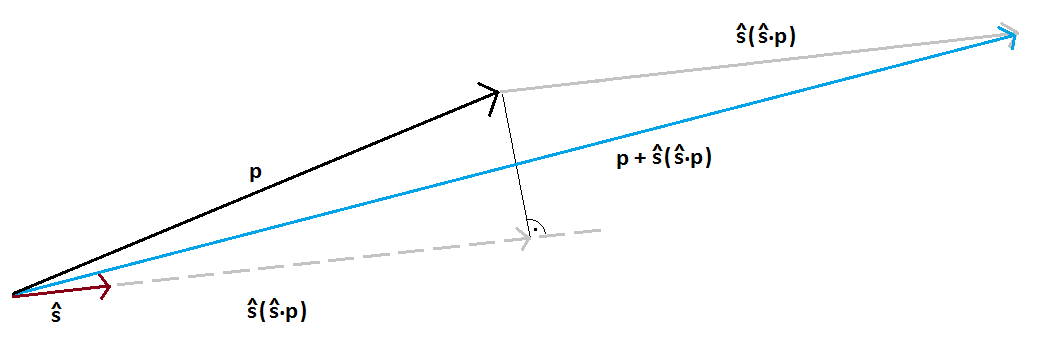
\includegraphics[width=0.9\textwidth]{arbitrary-axis-scale-diagram}
\caption{arbitrary axis scale}
\label{fig:arb_axis_scale}
\end{figure}

The resulting formula is this:
\begin{mdframed}
\[
	\mathbf{p\prime} = 
	\mathbf{p} + (\alpha - 1) \mathbf{\hat{s}}(\mathbf{\hat{s}}\cdot \mathbf{p})
\]
\end{mdframed}

Let's consider the special case when \(\mathbf{p}\perp\mathbf{\hat{s}}\). In that case \(\mathbf{\hat{s}}\cdot \mathbf{p} = 0\), so we get the following equation:
\[
	\mathbf{p\prime} = 
	\mathbf{p} + (\alpha - 1) \mathbf{\hat{s}}0 = \mathbf{p} + \mathbf{0} = \mathbf{p}
\]
I.e. \(\mathbf{p}\) is unaffected by the scaling operation, which is what we would expect.

Another interesting case is when \(\mathbf{p}\parallel\mathbf{\hat{s}}\). In that case \(\mathbf{\hat{s}}\cdot \mathbf{p} = |\mathbf{p}|\), which is the maximal value the expression can acquire, which means scaling does the most shift.

Let \(\mathbf{\hat{s1}}\perp\mathbf{\hat{s2}}\) or \(\mathbf{\hat{s1}}\parallel\mathbf{\hat{s2}}\). If we do two subsequent scale transformations on vector \(\mathbf{p}\) along each of the two axis the resulting point \(\mathbf{p\prime}\) the same regardless of the order of the operations. If none of the two conditions holds true then \(\mathbf{p\prime}\) will be more affected by the direction vector to be used for the first scaling operation. Given this, let \(\mathbf{\hat{x}}\perp\mathbf{\hat{y}}\perp\mathbf{\hat{z}}\); \(\mathbf{\hat{x}},\mathbf{\hat{y}},\mathbf{\hat{z}},\mathbf{\hat{p}} \in \mathbb{R}^3\) and \(\alpha,\beta\) and \(\gamma\) be scale actors along each vector respectively. We can combine 3 subsequent scaling operations in each direction into a single formula:
\[
	\mathbf{p\prime} = 
	\alpha \mathbf{\hat{x}}( \mathbf{p} \cdot \mathbf{\hat{x}}) +
	\beta \mathbf{\hat{y}}( \mathbf{p} \cdot \mathbf{\hat{y}}) +
	\gamma \mathbf{\hat{z}}( \mathbf{p} \cdot \mathbf{\hat{z}})
\]


\subsection{Deriving a matrix}

In the case where \(\mathbf{p},\mathbf{\hat{s}} \in \mathbb{R}^3\) we can decompose the arbitrary axis equation in the following system of 3 equations:
\begin{align*}
	p\prime_x = p_x + (\alpha - 1)s_x(s_x p_x +	s_y p_y + s_z p_z)	\\
	p\prime_y = p_y + (\alpha - 1)s_y(s_x p_x +	s_y p_y + s_z p_z)	\\
	p\prime_z = p_z + (\alpha - 1)s_z(s_x p_x +	s_y p_y + s_z p_z)
\end{align*}

We can rearrange each so that we have only one occurrence of \(p_x, p_y, p_z, p\prime_x, p\prime_y\) and \(p\prime_z\). And we get the following:
\begin{align*}
	p\prime_x = (1 + (\alpha - 1)s_x^2)p_x + (\alpha - 1)s_x s_y p_y + (\alpha - 1)s_x s_z p_z	\\
	p\prime_y = (\alpha - 1)s_y s_x p_x + (1 + (\alpha - 1)s_y^2)p_y + (\alpha - 1)s_y s_z p_z	\\
	p\prime_z = (\alpha - 1)s_z s_x p_x + (\alpha - 1)s_z s_y p_y + (1 + (\alpha - 1)s_z^2)p_z
\end{align*}

Extracting a homogeneous 3D matrix from the above system of equations is easy.
\[
	\begin{bmatrix}
	p\prime_x \\
	p\prime_y \\
	p\prime_z \\
	1
	\end{bmatrix}
	=	
	\begin{bmatrix}
	1 + (\alpha - 1)s_x^2 & (\alpha - 1)s_x s_y & (\alpha - 1)s_x s_z &  0  \\
	(\alpha - 1)s_x s_y & 1 + (\alpha - 1)s_y^2 & (\alpha - 1)s_y s_z &  0  \\
	(\alpha - 1)s_x s_z & (\alpha - 1)s_y s_z  & 1 + (\alpha - 1)s_z^2 & 0  \\
	0 & 0 & 0 &	1
	\end{bmatrix}
	\begin{bmatrix}
		p_x \\
		p_y \\
		p_z \\
		1
	\end{bmatrix}
\]


Now, let \(\mathbf{\hat{x}} =(1,0,0); \mathbf{\hat{y}} =(0,1,0); \mathbf{\hat{z}} =(0,0,1)\) and \(\alpha,\beta\) and \(\gamma\) be scale factors in each direction respectively. If we replaced \(\mathbf{\hat{s}}\) in the above matrix, with each and multiplied the 3 resulting matrices (after simplifying) we would get:
\[
	\mathbf{A} =
	\begin{bmatrix}
		\alpha & 0 & 0 & 0 \\
		0 &	1 & 0 & 0 \\
		0 & 0 & 1 &	0 \\
		0 & 0 & 0 &	1
	\end{bmatrix}
	\begin{bmatrix}
		1 & 0 & 0 & 0 \\
		0 &	\beta & 0 & 0 \\
		0 & 0 & 1 &	0 \\
		0 & 0 & 0 &	1
	\end{bmatrix}
	\begin{bmatrix}
		1 & 0 & 0 & 0 \\
		0 &	1 & 0 & 0 \\
		0 & 0 & \gamma &	0 \\
		0 & 0 & 0 &	1
	\end{bmatrix}
	=
	\begin{bmatrix}
		\alpha & 0 & 0 & 0 \\
		0 &	\beta & 0 & 0 \\
		0 & 0 & \gamma &	0 \\
		0 & 0 & 0 &	1
	\end{bmatrix}	
\]
Note that the order of the multiplication does not matter as \(\mathbf{\hat{x}}, \mathbf{\hat{y}}\) and \(\mathbf{\hat{z}}\) are mutually perpendicular.




%---------- 2.4. Reflect ---------
\section{Reflect}

Reflection is a linear operation, where a point \(\mathbf{p}\) is translated twice its distance to a reflector plane in a direction opposite to the normal vector of that plane. Consider the diagram \ref{fig:reflect}:

\begin{figure}[htb]
\centering
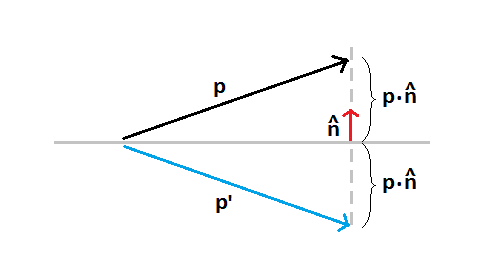
\includegraphics[width=0.9\textwidth]{reflection-diagram}
\caption{reflection}
\label{fig:reflect}
\end{figure}

The formula then becomes obvious:
\begin{mdframed}
\[
	\mathbf{p\prime} = 
	\mathbf{p} - 2\mathbf{\hat{n}}(\mathbf{\hat{n}} \cdot \mathbf{p})
\]
\end{mdframed}

If \(\mathbf{p}\) lies on the plane then \(\mathbf{\hat{n}} \cdot \mathbf{p} = 0\), so we get that \(\mathbf{p\prime} = \mathbf{p}\), which shouldn't be surprising. 

Another thing we might want to consider is when \(\mathbf{p}\) is behind the plane. In that case \(\mathbf{\hat{n}} \cdot \mathbf{p} < 0\) which means we'll be going in the direction of the plane normal (rather than it's opposite), so \(\mathbf{p\prime}\) will be in front of the plane. This also means that if we applied the same reflection transformation to a point twice (or any even number of times) we would get the same point.

An important thing to note is that we cannot define any plane simply by its normal direction, planes also have an offset from the origin as it could be expressed by the following plane equation:
\[
	A p_x + B p_y + C p_z + D = \mathbf{\hat{n}} \cdot \mathbf{p} + D = 0
\]
The above reflection equation assumes that \(D=0\). All we have to do to adapt it the formula to any plane is to translate the point \(\mathbf{p}\) by \(-D\mathbf{\hat{n}}\) (and effectively move the origin of the coordinate system to the plane) and then, after we reflect it, translate the resulting point \(\mathbf{p\prime}\) back by \(D\mathbf{\hat{n}}\).

\subsection{Deriving a matrix}
Deriving a 3D matrix is again quite easy. We first decompose the equation:
\begin{align*}
	p\prime_x = p_x - 2n_x(n_x p_x + n_y p_y + n_z p_z)		\\
	p\prime_y = p_y - 2n_y(n_x p_x + n_y p_y + n_z p_z)		\\
	p\prime_z = p_z - 2n_z(n_x p_x + n_y p_y + n_z p_z)		\\
\end{align*}

Then rearrange so that we only have one occurrence of \(p_x, p_y, p_z, p\prime_x, p\prime_y\) and \(p\prime_z\)and we arrive at:

\begin{align*}
	p\prime_x &= (1 - 2n_x^2)p_x -2n_x n_y p_y -2n_x n_z p_z	\\
	p\prime_y &= -2n_x n_y p_x + (1 - 2n_y^2)p_y -2n_y n_z p_z	\\
	p\prime_z &= -2n_x n_z p_x -2n_y n_z p_y + (1 - 2n_z^2)p_z	\\
\end{align*}

Which maps perfectly into a 3x3 matrix:

\[
	\begin{bmatrix}
	p\prime_x \\
	p\prime_y \\
	p\prime_z \\
	1
	\end{bmatrix}
	=	
	\begin{bmatrix}
		1 - 2n_x^2	&	-2n_x n_y	&	-2n_x n_z	&	0 \\
		-2n_x n_y	&	1 - 2n_y^2	& 	-2n_y n_z	&	0 \\
		-2n_x n_z	&	-2n_y n_z	&	1 - 2n_z^2	&	0 \\
		0 			&		0 		& 		0 		&	1
	\end{bmatrix}
	\begin{bmatrix}
		p_x \\
		p_y \\
		p_z \\
		1
	\end{bmatrix}
\]



%------ 2.5. Parallel Proj. ------
\section{Parallel Projection}
Parallel projection is a linear transformation which maps a point in a 3D scene onto a projection plane, where the distance of an object from the projection plane does not affect its appearance.

We could achieve the effect of parallel projection similarly to the reflection transformation discussed earlier. The only difference would be instead of going twice the distance in the direction opposite to the surface normal,
we go once. In other words using this formula:
\[
	\mathbf{p\prime} = 
	\mathbf{p} - \mathbf{\hat{n}}(\mathbf{\hat{n}} \cdot \mathbf{p})
\]

This would effectively translate \(\mathbf{p}\) onto the surface defined by the normal \(\mathbf{\hat{n}}\), but that is a special case of parallel projection called orthographic projection, because the projection ray is perpendicular to the surface (and coincides with the surface normal). In the general case however this will not necessarily be true, take a look at \ref{fig:parproj}.
\begin{figure}[htb]
\centering
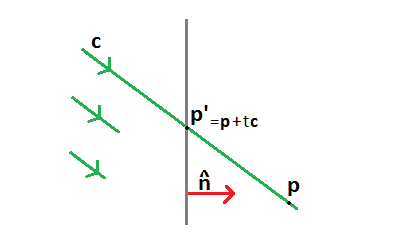
\includegraphics[width=0.9\textwidth]{projection-diagram}
\caption{parallel projection}
\label{fig:parproj}
\end{figure}
In this case \(\mathbf{c}\) the viewing direction is not parallel to the plane normal \(\mathbf{\hat{n}}\).

Because we know that \(\mathbf{p\prime}\) lies in the plane, so it must satisfy the plane equation:
\[
	\mathbf{p\prime} \cdot \mathbf{\hat{n}} + D = 0
\]
As with the reflection transform we will assume that the plane passes through the origin of the coordinate system (and will correct that later), which means we assume that \(D=0\).

We also know that the projected point \(\mathbf{p\prime}\) will lie on a line which goes trough the original point \(\mathbf{p}\) and has direction \(\mathbf{c}\), so it can be expressed as the result of the line equation:
\[
	\mathbf{p\prime} = \mathbf{p} + t\mathbf{c}
\]
Where \(t\) is a specific value we want to find. Replacing \(\mathbf{p\prime}\) back into the plane equation gives us:
\[
	(\mathbf{p} + t\mathbf{c}) \cdot \mathbf{\hat{n}} = 
	(\mathbf{p} \cdot \mathbf{\hat{n}}) + t(\mathbf{c} \cdot \mathbf{\hat{n}}) = 0
\]
And then we solve for \(t\):
\[
	t = -\frac{\mathbf{p} \cdot \mathbf{\hat{n}}}{\mathbf{c} \cdot \mathbf{\hat{n}}}
\]

Replacing \(t\) into the line equation gives us the parallel projection equation:
\begin{mdframed}
\[
	\mathbf{p\prime} = \mathbf{p} - \frac{\mathbf{p} \cdot \mathbf{\hat{n}}}{\mathbf{c} \cdot \mathbf{\hat{n}}} 
	\mathbf{c}
\]
\end{mdframed}


Now, lets consider orthographic projection again. When \(\mathbf{\hat{n}} \parallel \mathbf{c}\) it is also true that \(\mathbf{\hat{c}} = \frac{\mathbf{c}}{\mathbf{c} \cdot \mathbf{\hat{n}}} = \mathbf{\hat{n}}\). If we now specialized the equation we would get exactly our orthographic projection equation from before.


\subsection{Deriving matrix}

Following the standard procedure we decompose the equation into a system of three equation:

%p'x = px - (px*nx + py*ny + pz*nz)*cx/(cx*nx + cy*ny + cz*nz)
\begin{align*}
	p\prime_x = p_x - \frac	{p_x n_x + p_y n_y + p_z n_z}
							{\mathbf{\hat{n}}\cdot\mathbf{c}} cx	\\
	p\prime_y = p_y - \frac	{p_x n_x + p_y n_y + p_z n_z}
							{\mathbf{\hat{n}}\cdot\mathbf{c}} cy	\\
	p\prime_z = p_z - \frac	{p_x n_x + p_y n_y + p_z n_z}
							{\mathbf{\hat{n}}\cdot\mathbf{c}} cz	\\
\end{align*}

Then we rearrange and end up with three equations which look something like this:
\begin{align*}
	p\prime_x &=(1 - \frac{n_x c_x}{\mathbf{\hat{n}}\cdot\mathbf{c}}) p_x 
				   - \frac{n_y c_x}{\mathbf{\hat{n}}\cdot\mathbf{c}}  p_y
				   - \frac{n_z c_x}{\mathbf{\hat{n}}\cdot\mathbf{c}}  p_z
				\\
	p\prime_y &= - \frac{n_x c_y}{\mathbf{\hat{n}}\cdot\mathbf{c}}	p_x
			+(1 - \frac{n_y c_y}{\mathbf{\hat{n}}\cdot\mathbf{c}})	p_y
				 - \frac{n_z c_y}{\mathbf{\hat{n}}\cdot\mathbf{c}}	p_z
				\\
	p\prime_z &= - \frac{n_x c_z}{\mathbf{\hat{n}}\cdot\mathbf{c}}	p_x
				 - \frac{n_y c_z}{\mathbf{\hat{n}}\cdot\mathbf{c}}	p_y
			+(1 - \frac{n_z c_z}{\mathbf{\hat{n}}\cdot\mathbf{c}})	p_z
\end{align*}

And finally we construct our matrix:
\[
	\begin{bmatrix}
	p\prime_x \\
	p\prime_y \\
	p\prime_z \\
	1
	\end{bmatrix}
	=	
	\begin{bmatrix}
			1 - \frac{n_x c_x}{\mathbf{\hat{n}}\cdot\mathbf{c}}	
		&	- \frac{n_y c_x}{\mathbf{\hat{n}}\cdot\mathbf{c}}	
		&	- \frac{n_z c_x}{\mathbf{\hat{n}}\cdot\mathbf{c}}
		&	0
		\\
			- \frac{n_x c_y}{\mathbf{\hat{n}}\cdot\mathbf{c}}
		&	1 - \frac{n_y c_y}{\mathbf{\hat{n}}\cdot\mathbf{c}}
		&	- \frac{n_z c_y}{\mathbf{\hat{n}}\cdot\mathbf{c}}
		&	0
		\\
			- \frac{n_x c_z}{\mathbf{\hat{n}}\cdot\mathbf{c}}
		&	- \frac{n_y c_z}{\mathbf{\hat{n}}\cdot\mathbf{c}}
		&	1 - \frac{n_z c_z}{\mathbf{\hat{n}}\cdot\mathbf{c}}
		&	0
		\\
		0 & 0 & 0 & 1
	\end{bmatrix}
	\begin{bmatrix}
		p_x \\
		p_y \\
		p_z \\
		1
	\end{bmatrix}
\]

Notice that we divide by \(\mathbf{\hat{n}}\cdot\mathbf{c}\) in every cell and that \(-\) sign, we could factor these divisions into the \(w\) parameter and have something which looks much nicer and requires less operations.
\[
	\begin{bmatrix}
	p\prime_x \\
	p\prime_y \\
	p\prime_z \\
	p\prime_w
	\end{bmatrix}
	=	
	\begin{bmatrix}
			n_x c_x - \mathbf{\hat{n}}\cdot\mathbf{c}	
		&	n_y c_x
		&	n_z c_x
		&	0
		\\
			n_x c_y
		&	n_y c_y - \mathbf{\hat{n}}\cdot\mathbf{c}
		&	n_z c_y
		&	0
		\\
			n_x c_z
		&	n_y c_z
		&	n_z c_z - \mathbf{\hat{n}}\cdot\mathbf{c}
		&	0
		\\
		0 & 0 & 0 & -\mathbf{\hat{n}}\cdot\mathbf{c}
	\end{bmatrix}
	\begin{bmatrix}
		p_x \\
		p_y \\
		p_z \\
		1
	\end{bmatrix}
\]



%----- 2.6. Perspective Proj. ----
\section{Perspective Projection}

Perspective projection is a transformation in which 3D points are mapped onto a 2D surface (or plane). It has the property to affect the size of the projected objects (typically the further an object is the smaller its projection is). This projection is based on the pinhole camera model where all rays cross a projection plane and converge into a single point. Consider \ref{fig:persproj}: 
\begin{figure}[htb]
\centering
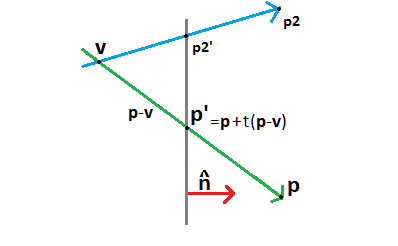
\includegraphics[width=0.8\textwidth]{persp-projection-diagram}
\caption{parallel projection}
\label{fig:persproj}
\end{figure}

It looks different to parallel projection and \ref{fig:parproj}, but also bares a lot of resemblance. The most significant difference is than instead of a constant viewing direction \(\mathbf{c}\) we now have a viewing direction that is different for every point. If we chose a focal point \(\mathbf{v}\) we can compute that viewing direction as \(\mathbf{p}-\mathbf{v}\). Then we can replace \(\mathbf{c}\) with the new direction and we end up with:
\begin{mdframed}
\[
	\mathbf{p\prime} = \mathbf{p} - \frac{\mathbf{p} \cdot \mathbf{\hat{n}}}{(\mathbf{p}-\mathbf{v}) \cdot \mathbf{\hat{n}}} 
	(\mathbf{p}-\mathbf{v})
\]
\end{mdframed}


\subsection{Deriving matrix}

Deriving a matrix is not so trivial this time, because the equation in not linear.


%---------- 2.3. Rotate ----------
\section{Rotate}


In the 2D sense rotation can be expressed by the formula
\[
	\mathbf{p\prime} = 
	\mathbf{\hat{x}}(\mathbf{\hat{x}} \cdot \mathbf{p})\cos\theta + \mathbf{\hat{y}}(\mathbf{\hat{y}} \cdot \mathbf{p})\sin\theta
\]
Where \(\mathbf{\hat{x}} \perp \mathbf{\hat{y}}\). 

Suppose we wanted to rotate a point \(\mathbf{p}\) at angle \(\theta\) which lies on a plane defined by the normal \(\mathbf{\hat{n}}\) (and for convenience passes through the origin). We need two perpendicular vectors on that plane to do the rotation - one is \(\mathbf{p}\) the other one we could obtain by \(\mathbf{p} \times \mathbf{\hat{n}}\), because we know that the product will it will be perpendicular \(\mathbf{p}\) by definition and we know that it will lie in the plane (because it is also perpendicular to \(\mathbf{\hat{n}}\)). So we obtain the following formula:
\begin{mdframed}
\[
	\mathbf{p\prime} = 
	\mathbf{p}\cos\theta + \mathbf{n}\times\mathbf{p}\sin\theta
\]
\end{mdframed}

What happens if \(\mathbf{p}\) does not lie on a plane passing though the origin? In that case we simply shift the coordinate system so that the origin lies on the plane (i.e. shift the original point \(\mathbf{p}\) in the opposite direction), and then after we do the operation we shift it back. A generic plane as already explained in previous sections is defined by a normal \(\mathbf{\hat{n}}\) and an offset value \(D\). To obtain \(D\) all we have to do is project \(\mathbf{p}\) onto \(\mathbf{\hat{n}}\).
Now that we have found \(D\) the translation vector we need to shift \(\mathbf{p}\) by is \(-D\mathbf{\hat{n}}\) and the translation vector we need to shift the result of the rotation is \(D\mathbf{\hat{n}}\).
We get two translations which look like this:
\begin{align*}
	\mathbf{p\prime} &=  \mathbf{p}-(\mathbf{p}\cdot\mathbf{\hat{n}})\mathbf{\hat{n}} \\
	\mathbf{p\prime\prime} &= \mathbf{p\prime}\cos\theta+\mathbf{n}\times\mathbf{p\prime}\sin\theta	\\
	\mathbf{p\prime\prime\prime} &= \mathbf{p\prime\prime}+(\mathbf{p}\cdot\mathbf{\hat{n}})\mathbf{\hat{n}}
\end{align*}

\subsection{Deriving a matrix}

Decomposing the 2D formula gives us:
\begin{align*}
	p\prime_x = p_x\cos\theta + (n_y p_z - n_z p_y)\sin\theta
	p\prime_y = p_y\cos\theta + (n_z p_x - n_x p_z)\sin\theta
	p\prime_z = p_z\cos\theta + (n_x p_y - n_y p_x)\sin\theta
\end{align*}

Rearranging gives us:
\begin{align*}
	p\prime_x &= p_x\cos\theta - n_z p_y\sin\theta + n_y p_z\sin\theta
	p\prime_y &= n_z p_x\sin\theta + p_y\cos\theta - n_x p_z\sin\theta
	p\prime_z &= -n_y p_x\sin\theta + n_x p_y\sin\theta + p_z\cos\theta
\end{align*}

So our matrix looks like this:
\[
	\begin{bmatrix}
	p\prime_x \\
	p\prime_y \\
	p\prime_z \\
	1
	\end{bmatrix}
	=
	\begin{bmatrix}
	\cos\theta		&	- n_z\sin\theta		&		n_y\sin\theta	&	0	\\
	n_z\sin\theta	&	\cos\theta			&		- n_x\sin\theta	&	0	\\
	-n_y\sin\theta	&	n_x\sin\theta		&		\cos\theta		&	0	\\
			0		&			0			&				0		&	1
	\end{bmatrix}
	\begin{bmatrix}
	p_x \\
	p_y \\
	p_z \\
	p_w
	\end{bmatrix}	
\]

And to account for the offset we need to do a translation matrices for:
\[
\mathbf{p\prime} =  \mathbf{p}-(\mathbf{p}\cdot\mathbf{\hat{n}})\mathbf{\hat{n}}
\]
and
\[
\mathbf{p\prime} =  \mathbf{p}+(\mathbf{p}\cdot\mathbf{\hat{n}})\mathbf{\hat{n}}
\]

Decomposition of the first gives us:
\begin{align*}
	p\prime_x &= p_x - (n_x p_x + n_y p_y + n_z p_z)		\\
	p\prime_y &= p_y - (n_x p_x + n_y p_y + n_z p_z)		\\
	p\prime_z &= p_z - (n_x p_x + n_y p_y + n_z p_z)		\\
\end{align*}

Rearranging that gives us:
\begin{align*}
	p\prime_x &= (1 - n_x) p_x - n_y p_y - n_z p_z		\\
	p\prime_y &= - n_x p_x + (1 -n_y) p_y + n_z p_z		\\
	p\prime_z &= - n_x p_x - n_y p_y + (1 - n_z) p_z	\\
\end{align*}

So our matrix looks like this:
\[
	\begin{bmatrix}
	p\prime_x \\
	p\prime_y \\
	p\prime_z \\
	1
	\end{bmatrix}
	=
	\begin{bmatrix}
	1 - n_x			&	- n_y		&	- n_z		&	0	\\
	- n_x			&	1 -n_y		&	- n_z		&	0	\\
	- n_x			&	- n_y		&	1 - n_z		&	0	\\
		0			&	0			&	0			&	1
	\end{bmatrix}
	\begin{bmatrix}
	p_x \\
	p_y \\
	p_z \\
	p_w
	\end{bmatrix}	
\]

The second equation would produce a similar matrix, but instead of minus there would be a plus sign.
\[
	\begin{bmatrix}
	p\prime_x \\
	p\prime_y \\
	p\prime_z \\
	1
	\end{bmatrix}
	=
	\begin{bmatrix}
	1 + n_x		&	n_y		&	n_z		&	0	\\
	n_x			&	1 +n_y	&	n_z		&	0	\\
	n_x			&	n_y		&	1 + n_z	&	0	\\
		0		&	0		&	0		&	1
	\end{bmatrix}
	\begin{bmatrix}
	p_x \\
	p_y \\
	p_z \\
	p_w
	\end{bmatrix}	
\]


%%%%%%%%%%% 3. Results %%%%%%%%%%%
\chapter{Results}           % chapter 3

%> SEG instruction to authors <%
\begin{quotation}
	``The results section contains applications of the methodology described above. The results of experiments
	(either physical or computational) are data and can be presented as tables or figures and analyses. Whenever
	possible, include at least one example of recorded data to illustrate the technology or concept being proposed.
	Case-history results are usually geologic interpretations.

	Selective presentation of results is important. Redundancy should be avoided, and results of minor variations on
	the principal experiment should be summarized rather than included. Details appearing in figure captions and
	table heads should not be restated in the text. In a well-written paper, the results section is often the
	shortest.''
\end{quotation}
%> SEG instruction to authors <%


Blah blah blah





%%%%%%%%%% 4. Conclusion %%%%%%%%%
\chapter{Conclusion}		% chapter 4

%> SEG instruction to authors <%
\begin{quotation}
	``The conclusion section should include (1) principles, relationships, and generalizations inferred from the
	results (but not a repetition of the results); (2) any exceptions to or problems with those principles,
	relationships, and generalizations, as indicated by the results; (3) agreements or disagreements with previously
	published work; (4) theoretical implications and possible practical applications of the work; and (5) conclusions
	drawn (especially regarding significance). In particular, with reference to item (1) above, a conclusion that
	only summarizes the results is not acceptable.''
\end{quotation}
%> SEG instruction to authors <%


Blah blah blah






%%%%%%%%%% Bibliography %%%%%%%%%%
\begin{thebibliography}{9}
  % type bibliography here
\end{thebibliography}





\end{document}